\documentclass[tikz,border=6pt]{standalone}

\usepackage[T1]{fontenc}
\usepackage[utf8]{inputenc}
\usepackage{tikz}
\usetikzlibrary{positioning,arrows.meta}

\begin{document}
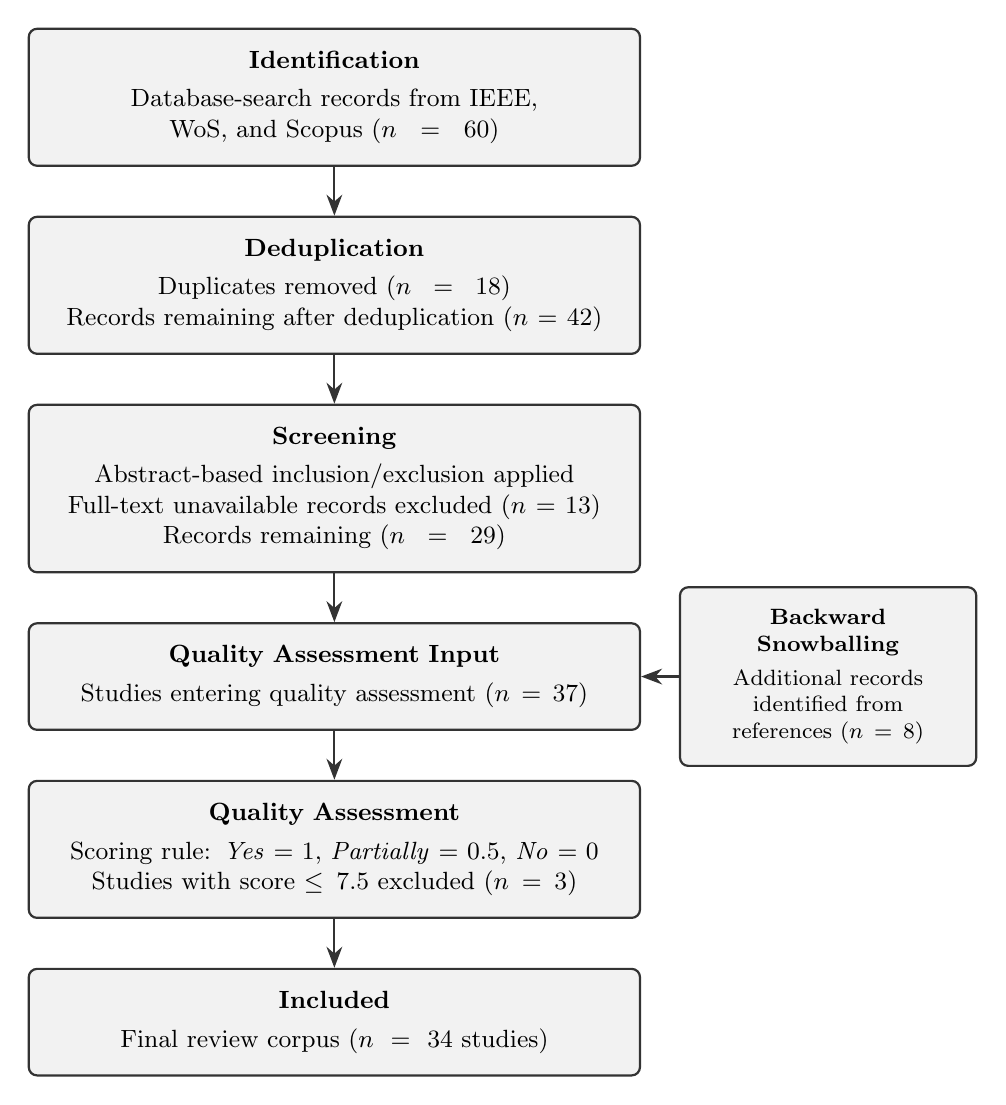
\begin{tikzpicture}[
    node distance = 0.62cm and 0.48cm,
    mainbox/.style = {
        rectangle,
        draw=black!80,
        thick,
        fill=black!5,
        text width=7.2cm,
        align=center,
        rounded corners=3pt,
        inner sep=8pt,
        font=\small
    },
    sidebox/.style = {
        rectangle,
        draw=black!80,
        thick,
        fill=black!5,
        text width=3.2cm,
        align=center,
        rounded corners=3pt,
        inner sep=8pt,
        font=\footnotesize
    },
    arrow/.style = {
        -{Stealth[scale=1.15]},
        thick,
        draw=black!80
    }
]

\node (id) [mainbox] {\textbf{Identification}\\[3pt] Database-search records from IEEE, WoS, and Scopus ($n=60$)};

\node (dedup) [mainbox, below=of id] {\textbf{Deduplication}\\[3pt] Duplicates removed ($n=18$)\\ Records remaining after deduplication ($n=42$)};

\node (screen) [mainbox, below=of dedup] {\textbf{Screening}\\[3pt] Abstract-based inclusion/exclusion applied\\ Full-text unavailable records excluded ($n=13$)\\ Records remaining ($n=29$)};

\node (qain) [mainbox, below=of screen] {\textbf{Quality Assessment Input}\\[3pt] Studies entering quality assessment ($n=37$)};

\node (qa) [mainbox, below=of qain] {\textbf{Quality Assessment}\\[3pt] Scoring rule: \textit{Yes} = 1, \textit{Partially} = 0.5, \textit{No} = 0\\ Studies with score $\le 7.5$ excluded ($n=3$)};

\node (inc) [mainbox, below=of qa] {\textbf{Included}\\[3pt] Final review corpus ($n=34$ studies)};

\node (snow) [sidebox, right=of qain] {\textbf{Backward Snowballing}\\[3pt] Additional records\\ identified from\\ references ($n=8$)};

\draw [arrow] (id) -- (dedup);
\draw [arrow] (dedup) -- (screen);
\draw [arrow] (screen) -- (qain);
\draw [arrow] (qain) -- (qa);
\draw [arrow] (qa) -- (inc);
\draw [arrow] (snow) -- (qain);

\end{tikzpicture}
\end{document}
